\begin{figure}[H]
    \centering
    \begin{subfigure}{\textwidth}
        \centering
        % include second image
        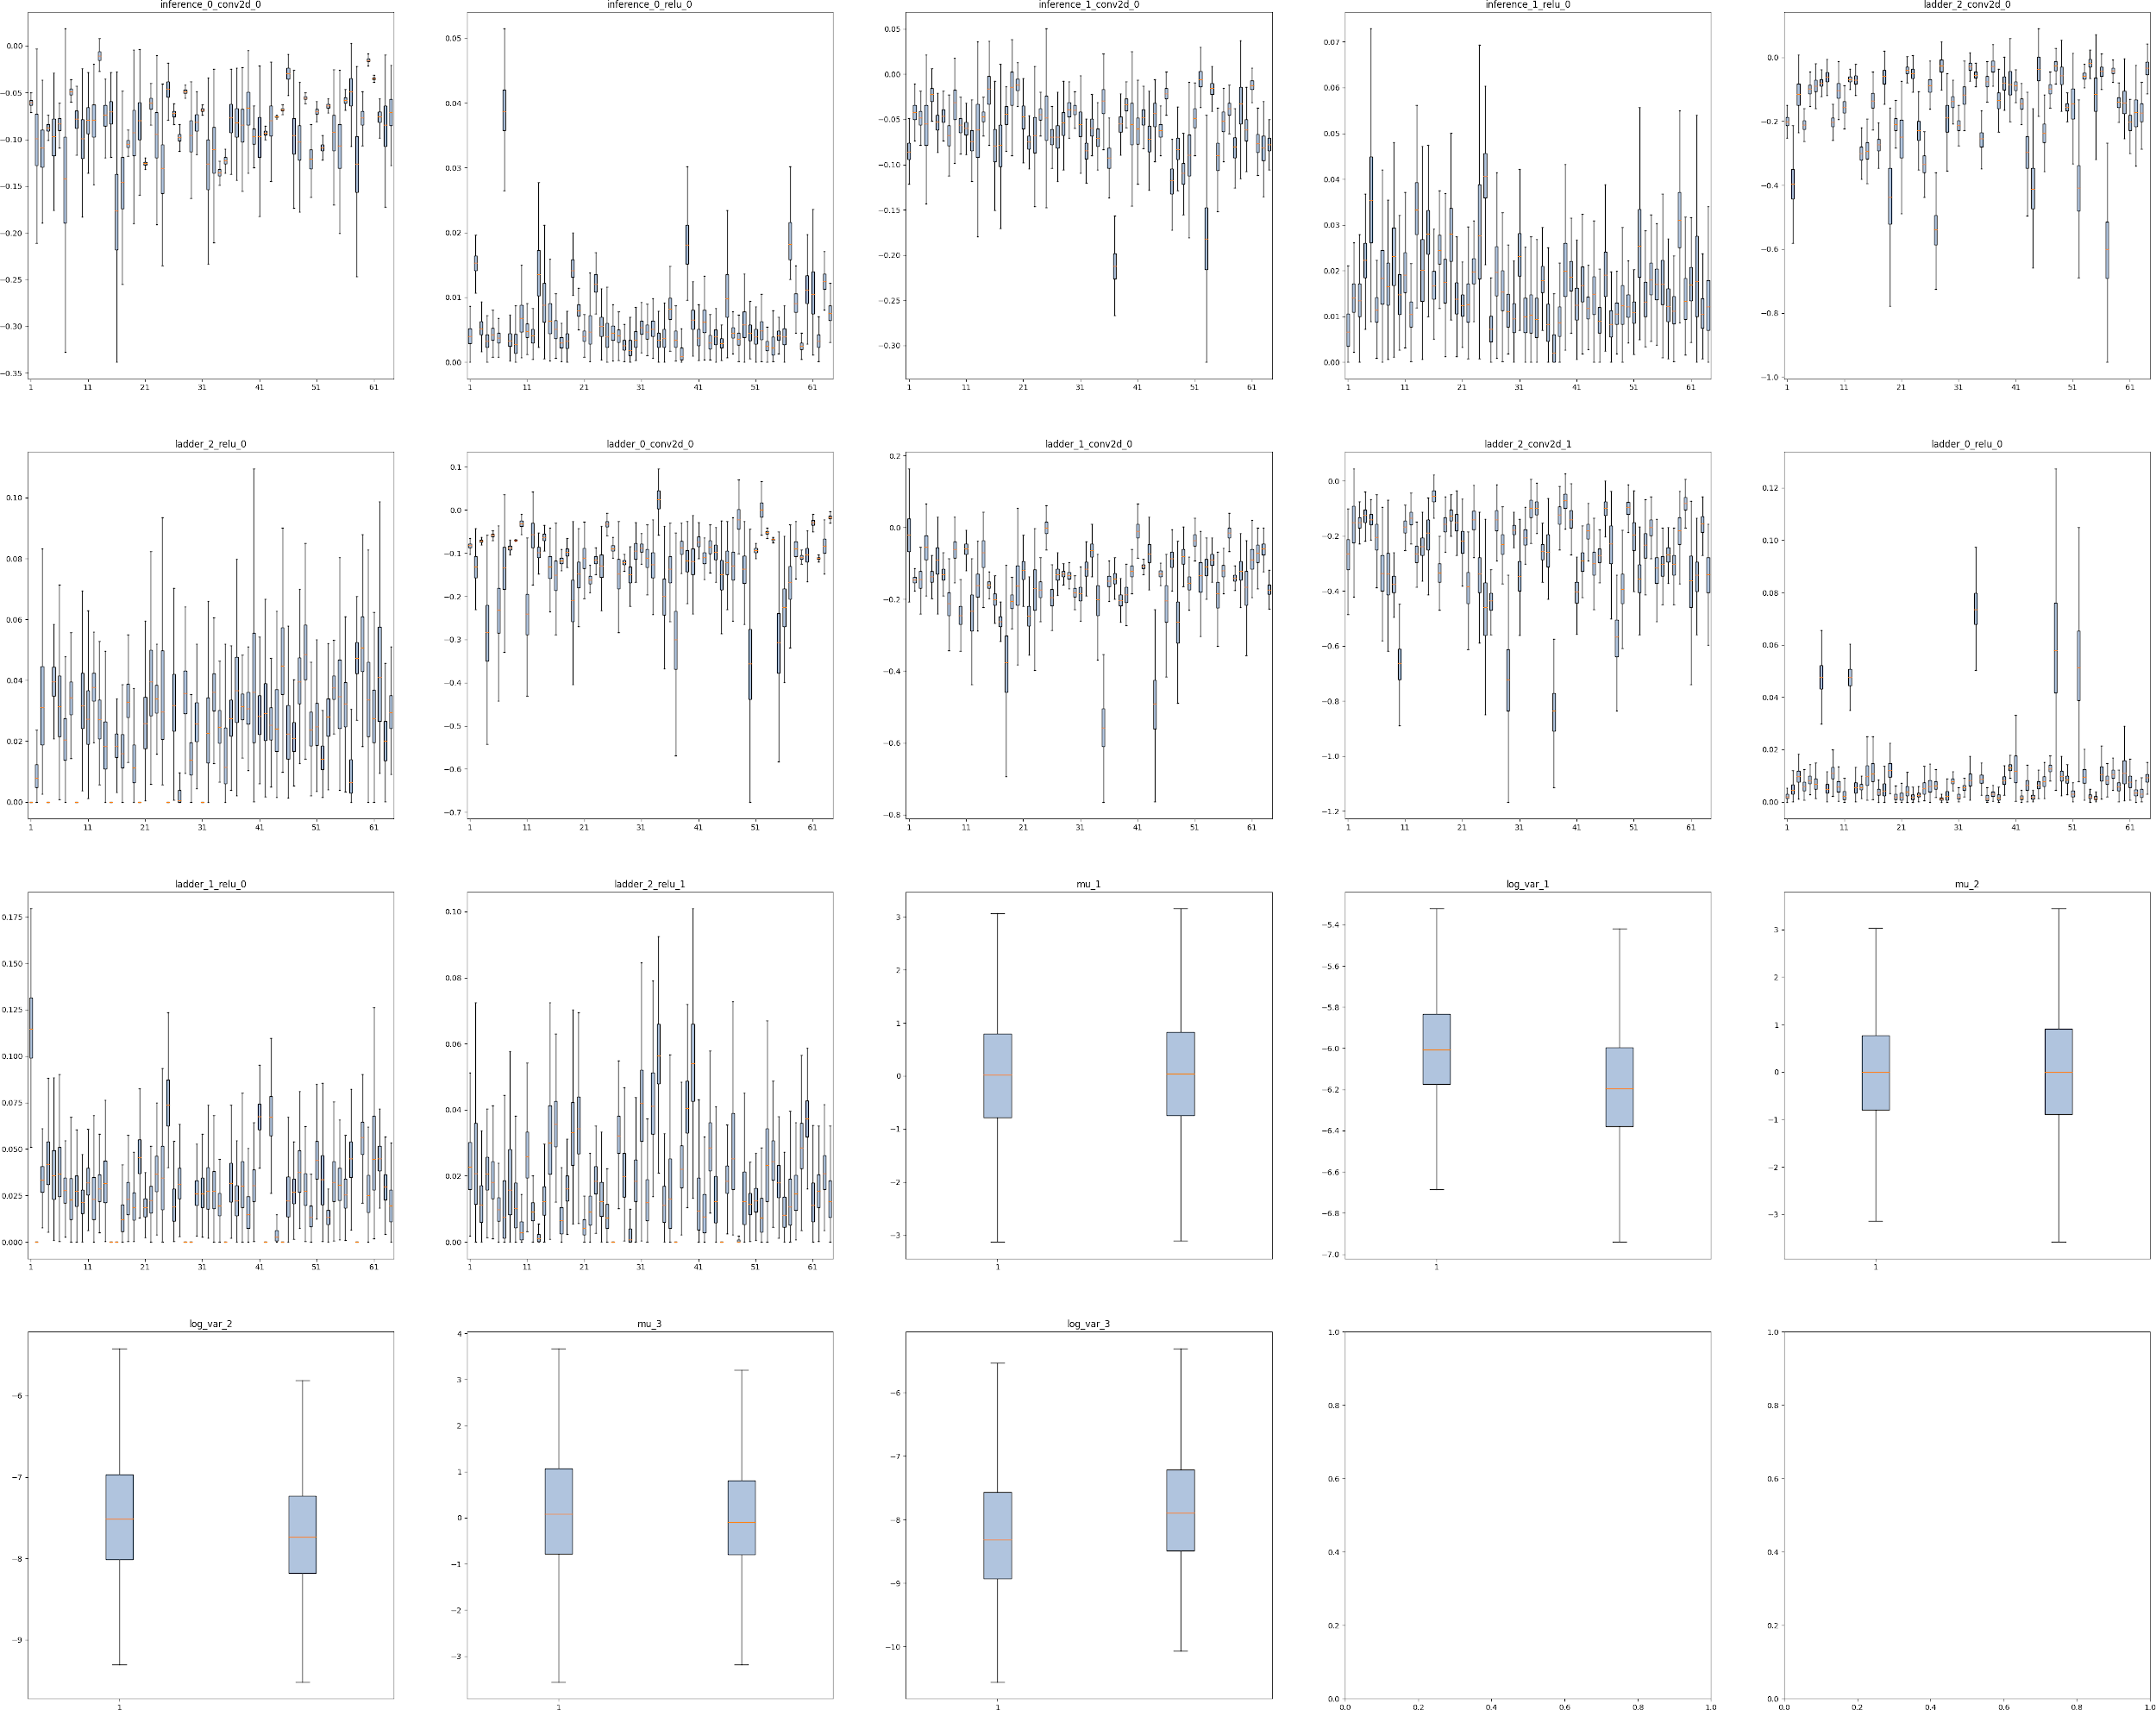
\includegraphics[height=.8\textheight]{images/sparseness/encoder_fm1_fms.png}
    \end{subfigure}
    \caption[\textsc{Mnist}-VLAE-factor-1: Feature Map Activites]{Feature map activities for \textsc{Mnist}-\ac{VLAE}-factor-1.
    Each boxplot corresponds to the distribution of the mean value of one feature map after the convolution.
    }
\end{figure}

\begin{figure}[H]
    \centering
    \begin{subfigure}{\textwidth}
        \centering
        % include second image
        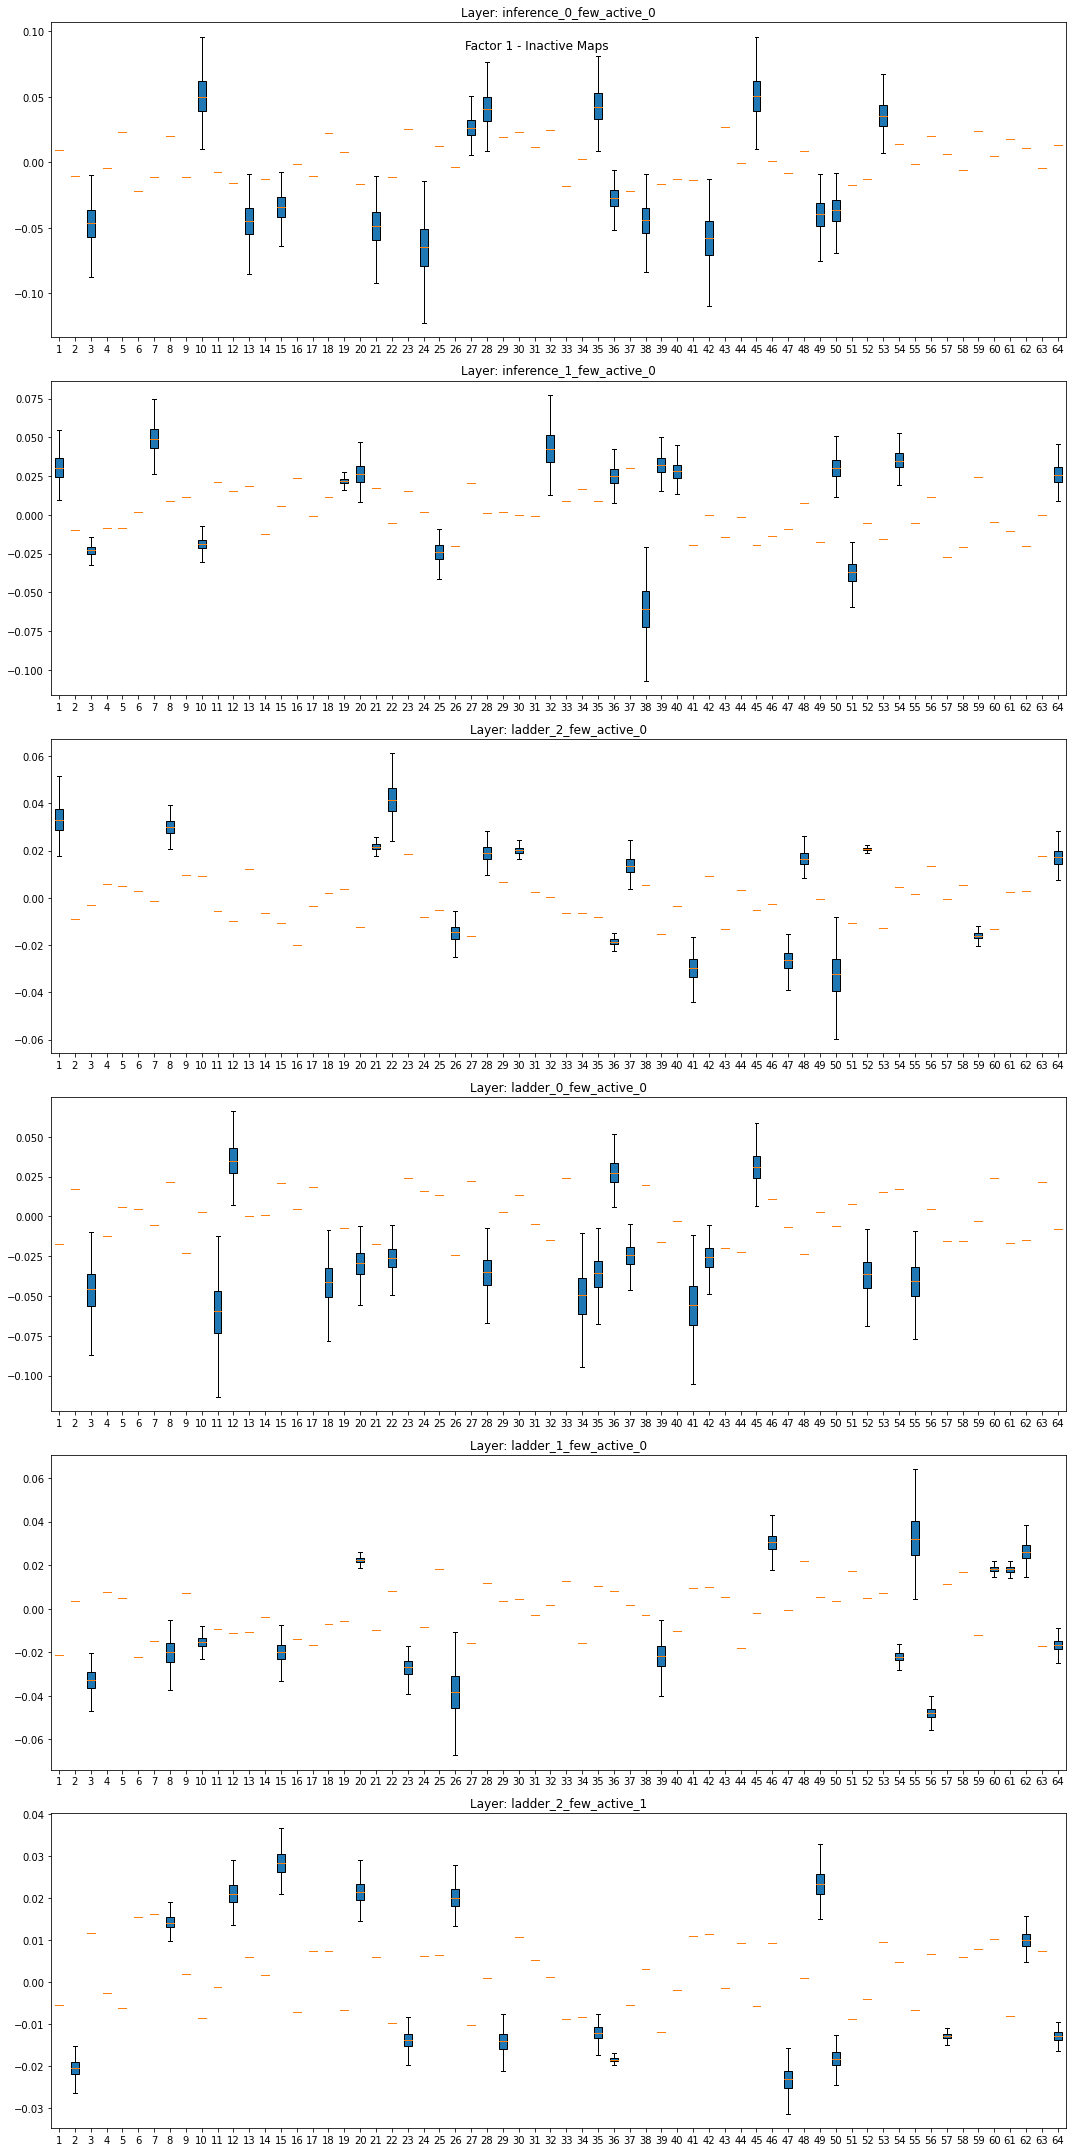
\includegraphics[height=.8\textheight]{images/sparseness/encoder_fm1_fms_inactive.png}
    \end{subfigure}
    \caption[\textsc{Mnist}-VLAE-factor-1: Most Active Feature Maps]{Activities of only the $\left \lceil \frac{n}{4} \right \rceil$ most active feature maps in \textsc{Mnist}-\ac{VLAE}-factor-1.
    Each boxplot corresponds to the distribution of the mean value of one feature map after the convolution.
    Less active feature maps are set to their mean values.
    }
\end{figure}

\begin{figure}[H]
    \centering
    \begin{subfigure}{\textwidth}
        \centering
        % include second image
        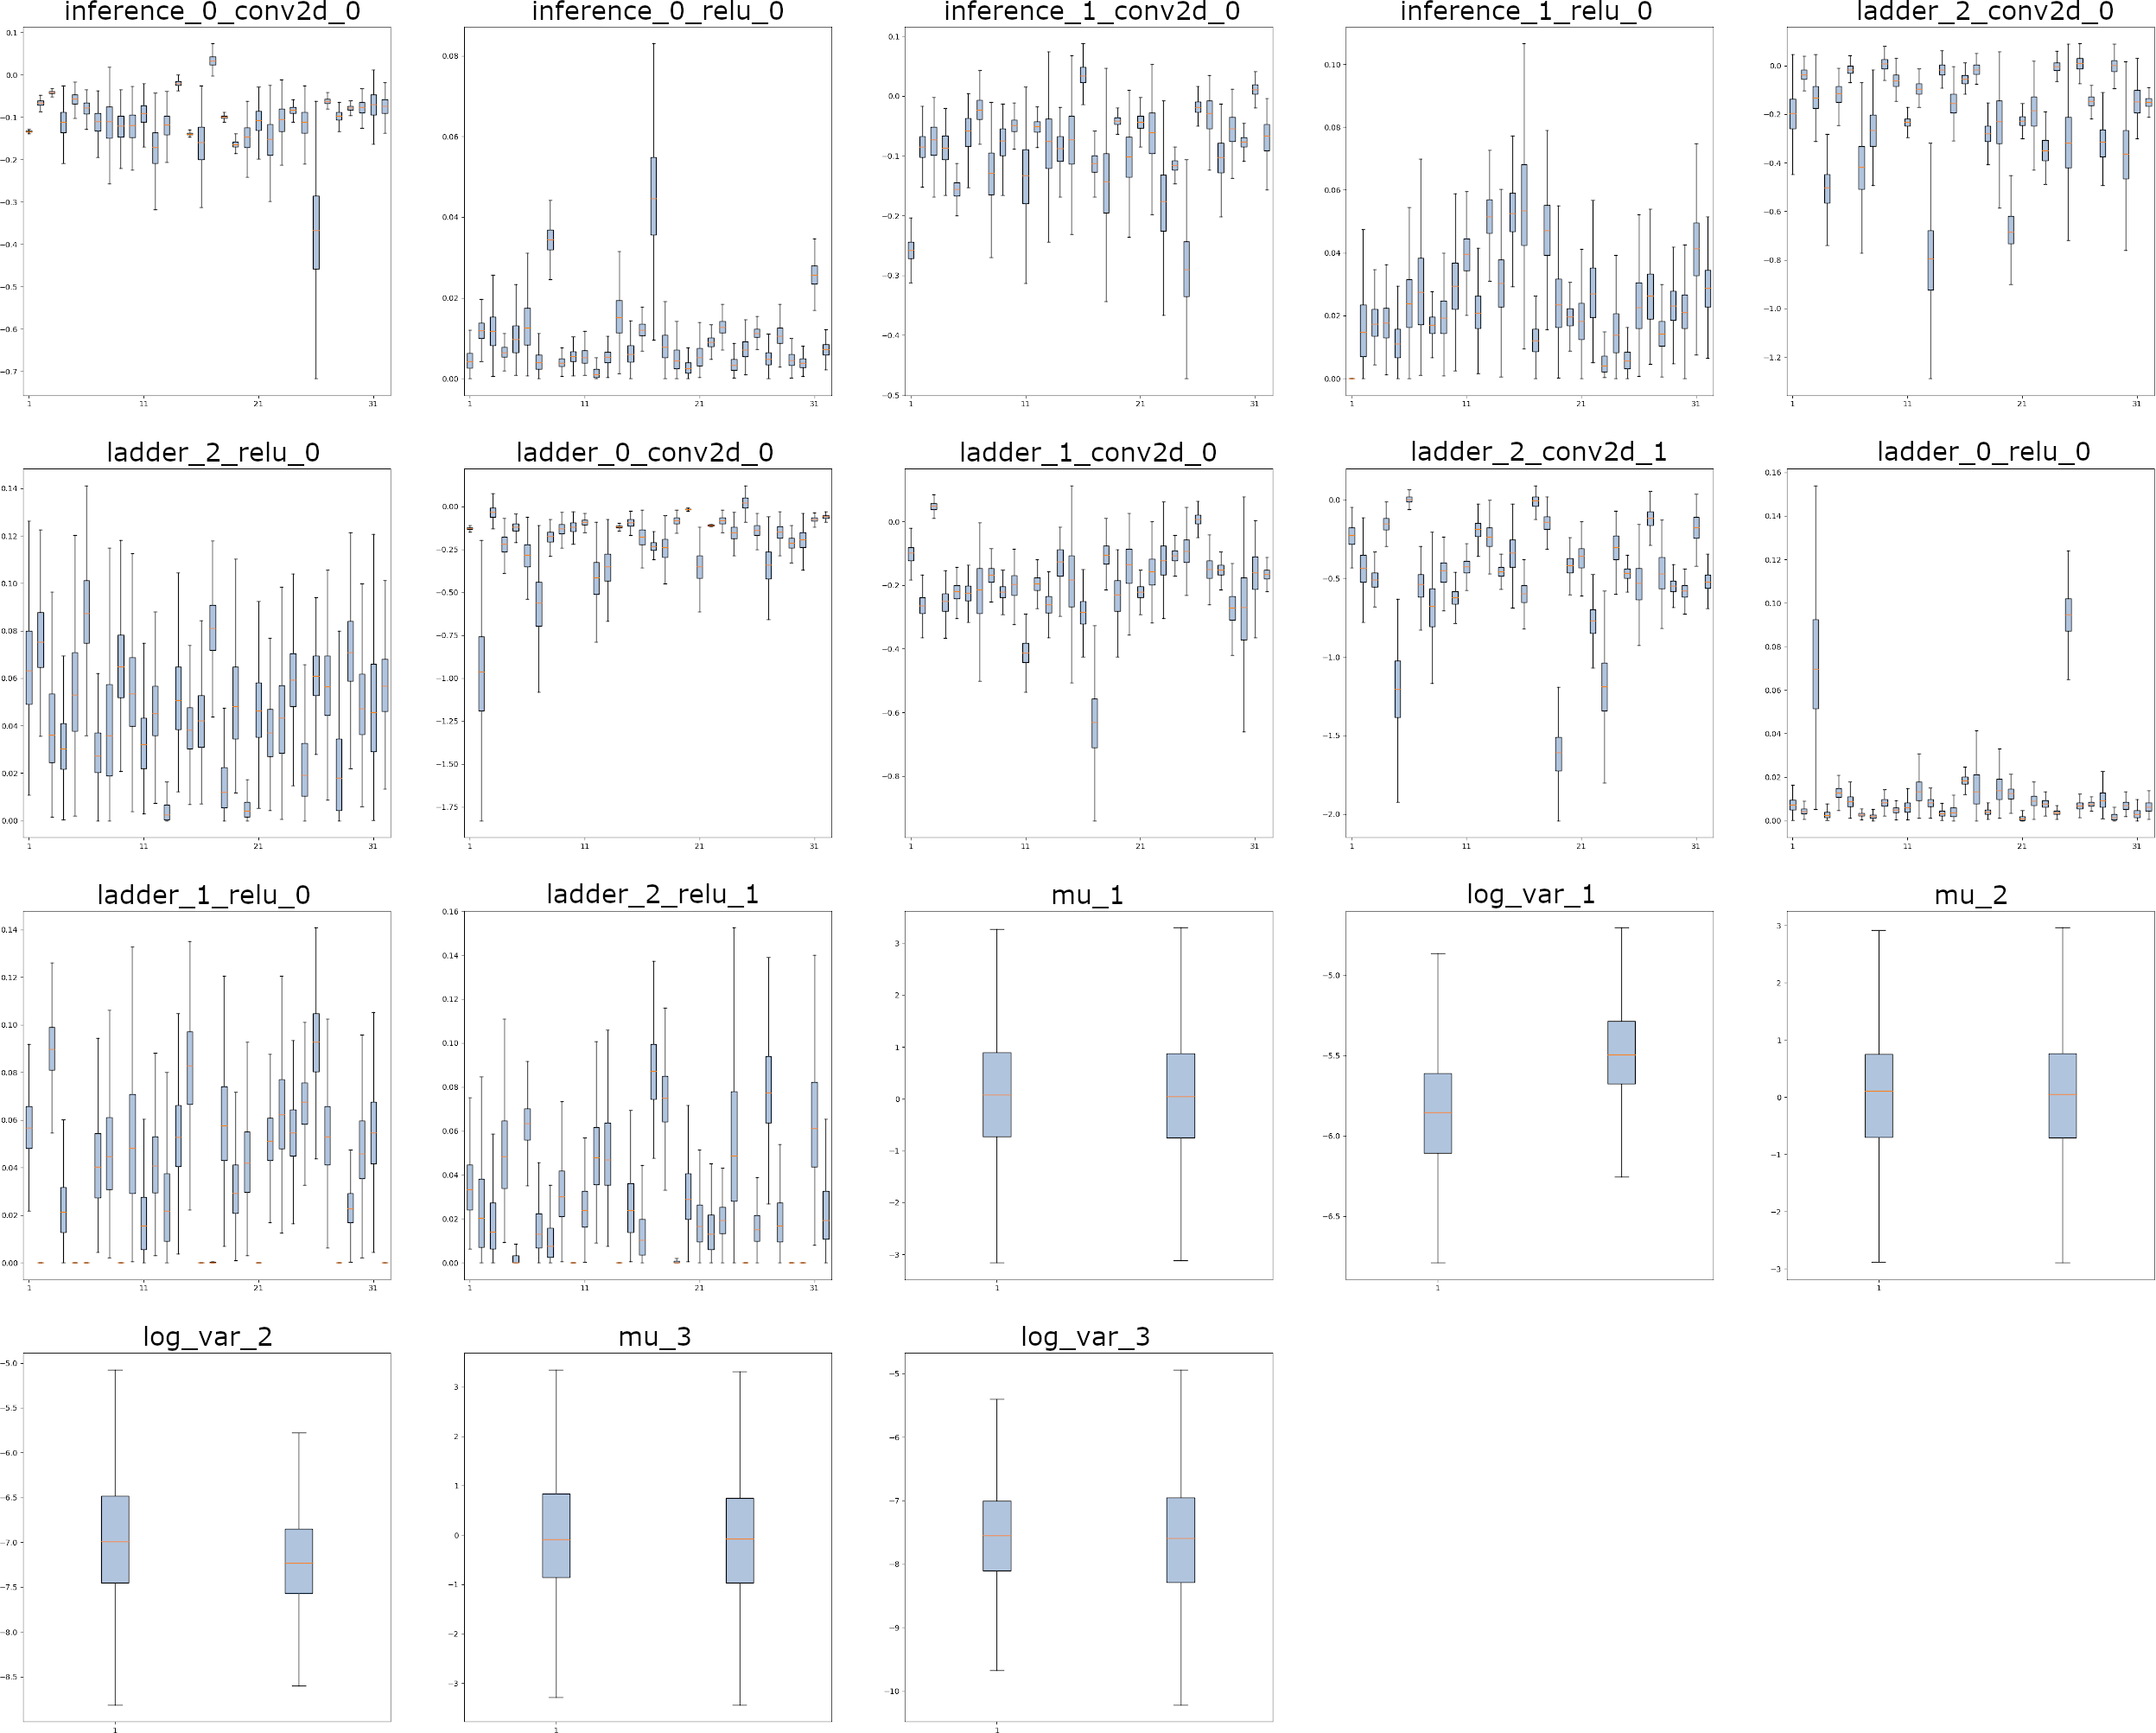
\includegraphics[height=.8\textheight]{images/sparseness/encoder_fm2_fms.png}
    \end{subfigure}
    \caption[\textsc{Mnist}-VLAE-factor-2: Feature Map Activites]{Feature map activities for \textsc{Mnist}-\ac{VLAE}-factor-2.
    Each boxplot corresponds to the distribution of the mean value of one feature map after the convolution.
    }
\end{figure}

\begin{figure}[H]
    \centering
    \begin{subfigure}{\textwidth}
        \centering
        % include second image
        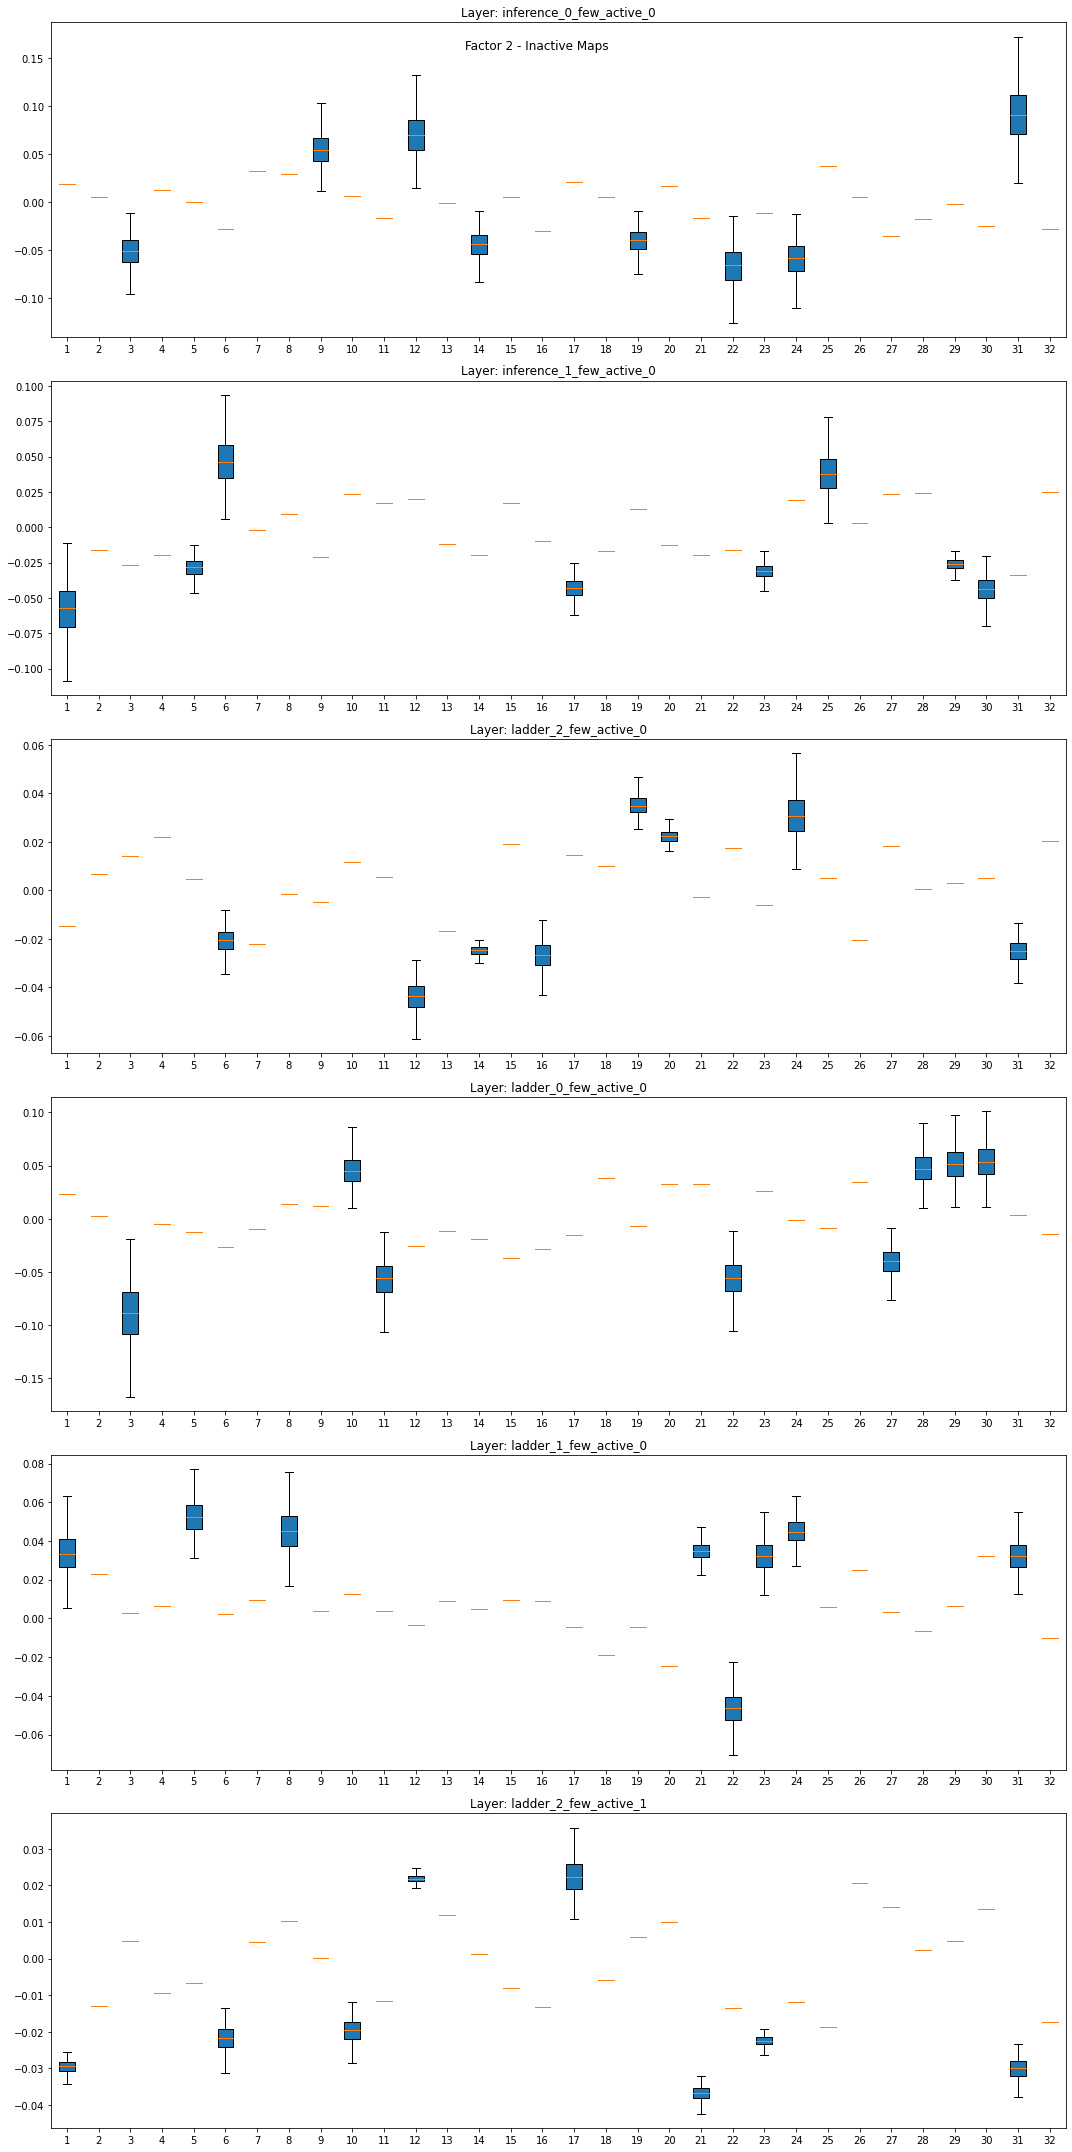
\includegraphics[height=.8\textheight]{images/sparseness/encoder_fm2_fms_inactive.png}
    \end{subfigure}
    \caption[\textsc{Mnist}-VLAE-factor-2: Most Active Feature Maps]{Activities of only the $\left \lceil \frac{n}{4} \right \rceil$ most active feature maps in \textsc{Mnist}-\ac{VLAE}-factor-2.
    Each boxplot corresponds to the distribution of the mean value of one feature map after the convolution.
    Less active feature maps are set to their mean values.
    }
\end{figure}